\chapter{The LHCb experiment}
\label{ch:lhcb}

The following chapter first introduces the \lhc and the \lhcb detector before briefly
describing data collection and processing.
This will include a description of \pid at the \lhcb detector, triggering and event simulation.



%%%%%%%%%%%%%%%%%%%%%%%%%%%%%%%%%%%%%%%%%%%%%%%%%%%%%%%%%%%%%%%%%%%%%%%%%%%%%%%%
\section{The LHC}
The \lhc is a superconducting synchrotron which can simultaneously accelerate beams of proton bunches
in opposite directions.
Physically, the \lhc is located at \cern, near Geneva, Switzerland; it is 27\km in
circumference and spans the Franco-Swiss border at a depth of about 100\m.
Protons are supplied to the \lhc from the \sps with an energy of 450\gev, they can then
be accelerated and collided with a design centre of mass energy of 14\tev.
In the years 2011 and 2012 the centre of mass energy was 7 and $8\tev$ respectively.
Once the desired energy is reached the beams are collided at four interaction points, \lhcb is
situated at one of them.
Collisions of proton bunches occur every 50\ns reaching luminosities of up to
$7\e{33}\,\mathrm{cm}^{2}\mathrm{s}^{-1}$, however the beams entering \lhcb must be defocused, to
$3(4)\e{33}\,\mathrm{cm}^{2}\mathrm{s}^{-1}$ in 2011(2012), in order to reduce occupancy in the
\lhcb detector.
These high energy collisions produce a vast number of \bbbar pairs which subsequently hadronize
into \bquark hadrons, it is the prospect of studying these bound states of \bquark (and other heavy
flavour) quarks that has motivated the design of the \lhcb detector.



\chapter{The LHCb detector / Experimental}
\label{ch:lhcb}

The following chapter first introduces the \lhc and the \lhcb detector before going on to briefly
describe data collection and processing.
This will include a description of \pid at the \lhcb detector, triggering and event simulation.



%%%%%%%%%%%%%%%%%%%%%%%%%%%%%%%%%%%%%%%%%%%%%%%%%%%%%%%%%%%%%%%%%%%%%%%%%%%%%%%%
\section{The \lhc}
The \lhc is a $27\km$ circumference particle accelerator which spans the Franco-Swiss border, and
is the most recent addition to \cern's accelerator complex, and is designed to accelerate protons
upto $14\tev$ and collide them.
Protons are delivered to the \lhc synchrotron ring by from the \sps with an energy of $450\gev$.
They are then accelerated such that they collide with a centre-of-mass energy of $8(7)\tev$ in
2012(2011) and a maximum luminosity of $2\e{32}\,\mathrm{cm}^{-2}\mathrm{s}^{-1}$.
Particles are collided at four interaction points where the detectors \atlas, \alice, \cms and
\lhcb are located.


%Protons and heavy ions are injected into the \lhc at $450\gev$ from the \sps, and then accelerated
%to energies on the \tev scale before colliding them at one of four interaction points around the
%ring.
%The \lhc is designed to collide protons every $25\ns$ with a centre-of-mass energy of $14\tev$,
%however in Run 1 it ran at $50\ns$ and collided particles with energies of 7 and $8\tec$ in 2011
%and 2012 respectively.




%Typically a 2012 (2011) fill of the \lhc collided protons with a centre-of-mass energy of $8(7)\tev$
%every $50\ns$ with a maximum luminosity of $2\e{32}\,\mathrm{cm}^{-2}\mathrm{s}^{-1}$.
%Particles are injected into the \lhc with an energy of 450\gev, where they are then accelerated
%up to the desired energy.




%%%%%%%%%%%%%%%%%%%%%%%%%%%%%%%%%%%%%%%%%%%%%%%%%%%%%%%%%%%%%%%%%%%%%%%%%%%%%%%%
\section{The \lhcb detector}

Modern high energy flavour physics experiments usually study the decays of particles containing
\bquark or \cquark quarks.
These paritcles typically travel around $\cm$ before decaying into some combination of leptons and
hadrons.
A detector designed for flavour physics, therefore, must be able to resolve decay vertices
at which \bquark and \cquark containing hadrons decay, and then reconstruct and identify the particles
into which they decay.
The \lhcb detector is just such an apparatus, where the above requirements drove its design.
\lhcb is a single-arm forward spectrometer, meaning that while
the reconstruction of non-interacting particles, such as neutrinos, is difficult, there is room for
a precise vertex detector and \pid systems which are absent from modern general purpose detectors.

%Detector geometry and subdetector layout are shown in Fig.~\ref{fig:lhcb:lhcb},
Figure~\ref{fig:lhcb:lhcb} shows the \lhcb detector layout with subdetector systems indicated.
The \lhcb $z$ coordinate is defined by the \lhc beam pipe which passes through the centre of the
detector, the $x$ and $y$ coordinates are then the horizontal and vertical axes respectively.
After the interaction point detected particles travel in the forward $z$ direction (downstream) through the
detector volume.
Part of this is immersed in a magnetic field with an integrated field strengh of $4\,\mathrm{Tm}$,
this bends charged particles in the $x$ direction

where charged particles are bent in the $x$ plane by a conventional magnet.
This magnet is
the detector in a magnetic field which has an integrated field strength of $4\,\mathrm{Tm}$.
The various subdetector systems trough which particles pass can be broadly categorized as tracking,
particle identification or calorimetry.


\begin{figure}
  \begin{center}
    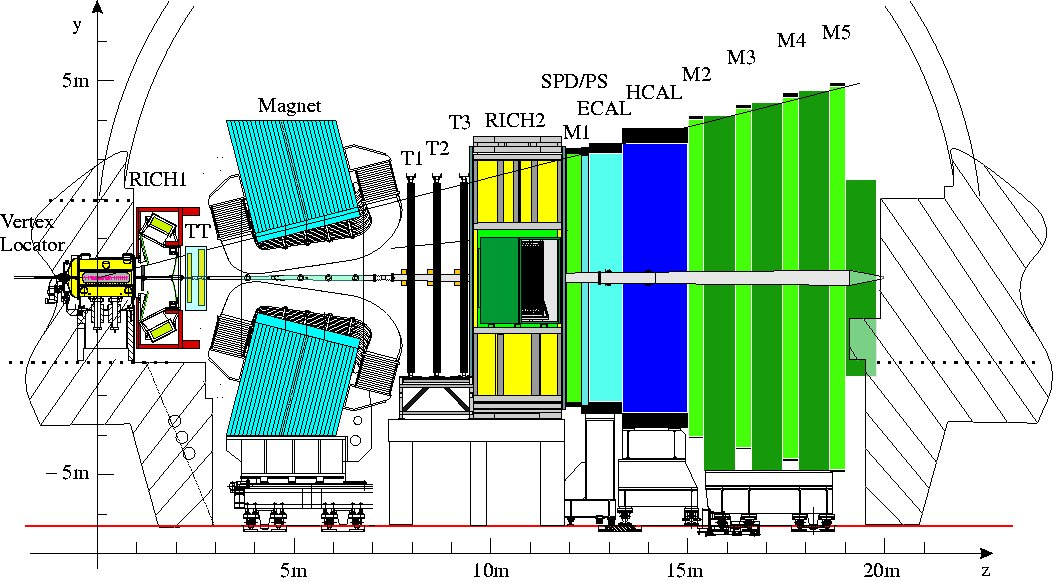
\includegraphics[width=\textwidth]{LHCb_detector}
  \end{center}
  \caption[\lhcb detector]
  {\small
    Schematic diagram of the \lhcb detector showing subdetector systems.
  }
  \label{fig:lhcb:lhcb}
\end{figure}

%Tracking begins close to the interaction point with the Vertex Locator (\velo), the aim of which is
%to resolve tracks in such a high occupancy region.
%Charged particles traveling in the detection region will then be observed as deposits in the Tracker
%Turicensis (\ttracker) before the magnet, and the three tracking stations (\Tone, \Ttwo and
%\Tthree) after the magnet.
%Particle identification information primarily comes from the two Ring Imaging Cherenkov (\rich)
%detectors, which allow separation between pions, kaons and protons.
%Calorimeters measure the energy of electrons, photons and hadrons.
%The muon stations provide tracking information for particles which penetrate the calorimeter
%systems, and therefore also provide particle identification for muons.

In the high energy proton-proton collisions provided by the \lhc \bbbar pairs are produced in such
away that their momentum vectors point along the beam axis; this is shown in shown in
Fig.~\ref{fig:lhcb:bbbar}.
This motivates the \lhcb detector's asymmetric design, the acceptance being from
$15\mrad$ to £$300(250)\mrad$ in the bending (non-bending) plane.
This equates in pseudo-rapidity, $\eta$, to approximately $2<\eta<5$ where:
\begin{equation}
  \eta = -\log\left(\tan\frac\theta2\right),
\end{equation}
and $\theta$ is the angle between a particle's momentum vector and the positive $z$ direction.
This detection region is sufficient to cover nearly 50\% of \bquark quarks produced.
%The asymmetric design of the \lhcb detector is unique among high energy physics experiments...

\begin{figure}
  \begin{center}
    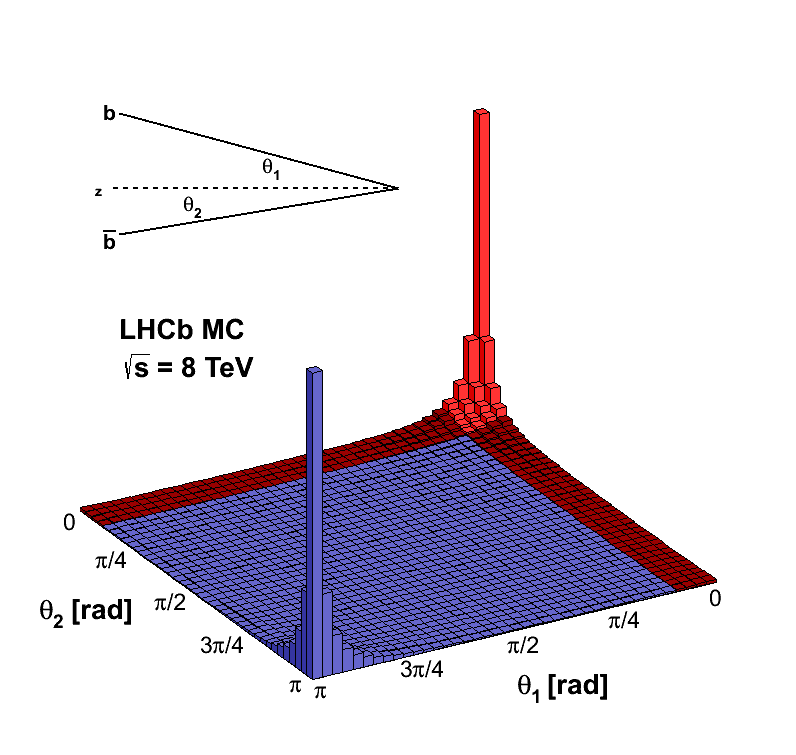
\includegraphics[width=0.5\textwidth]{acceptance}
  \end{center}
  \caption[Simulated production of \protect\bbbar pairs]
  {\small
    Simulation of the production of \bquark and \protect\bquarkbar quarks with angles $\theta_1$ and
    $\theta_2$ from the beam axis respectively.
    The full plot would be detected in a general purpose detector and the red area is that covered
    by the \lhcb detector.
  }
  \label{fig:lhcb:bbbar}
\end{figure}



%%%%%%%%%%%%%%%%%%%%%%%%%%%%%%%%%%%%%%%%%%%%%%%%%%%%%%%%%%%%%%%%%%%%%%%%%%%%%%%%
\subsection{Tracking}
The proton-proton interaction point is surrounded by the \velo.
This is a very high multiplicity region and therefore a high resolution required is provided by the
\velo.
Resolving tracks here is not only important to identify the primary vertex (PV), but also the
secondary vertex indicative of long lived particles that decay via the Weak interaction, which is
vitally important for the \lhcb physics program.
The \velo enables this by getting very close to the beam line and a high resolution, courtesy of
silicon strip detection layers working in $(r,\phi)$ coordinates.

There are 42 of each the $r$ and $\phi$ sensors in the \velo, organized into 21 detection layers,
with an additional four $r$ upstream sensors for pile-up veto.
\bam{Pile-up veto here.}
Each of these layers is split into two haves which can retract during \lhc beam injection, and then
close when beams are declared stable.
This movement allows the detection region to begin $8\mm$ from the beam centre, reducing track
extrapolation back to the primary vertex.
Particles emerging from the primary vertex in the range $1.6<\eta<4.9$, and $|z|<10.6\cm$ can be
detected in the \velo.
The pitch of the silicon strips varies from $\sim40\mum$ closest to the beam, to $\sim100\mum$
and has an impact resolution of $20\mum$ for high momentum tracks.
The geometry of the \velo is shown in Fig.~\ref{fig:lhcb:velo}.

%The tracking system begins with the \velo.
%Resolving tracks coming from the interaction region is vitally important for the \lhcb physics
%program.
%The \velo surrounds the interaction region with high resolution silicon strip detectors with
%cylindrical $(r,\phi)$ coordinates.

\begin{figure}
  \begin{center}
    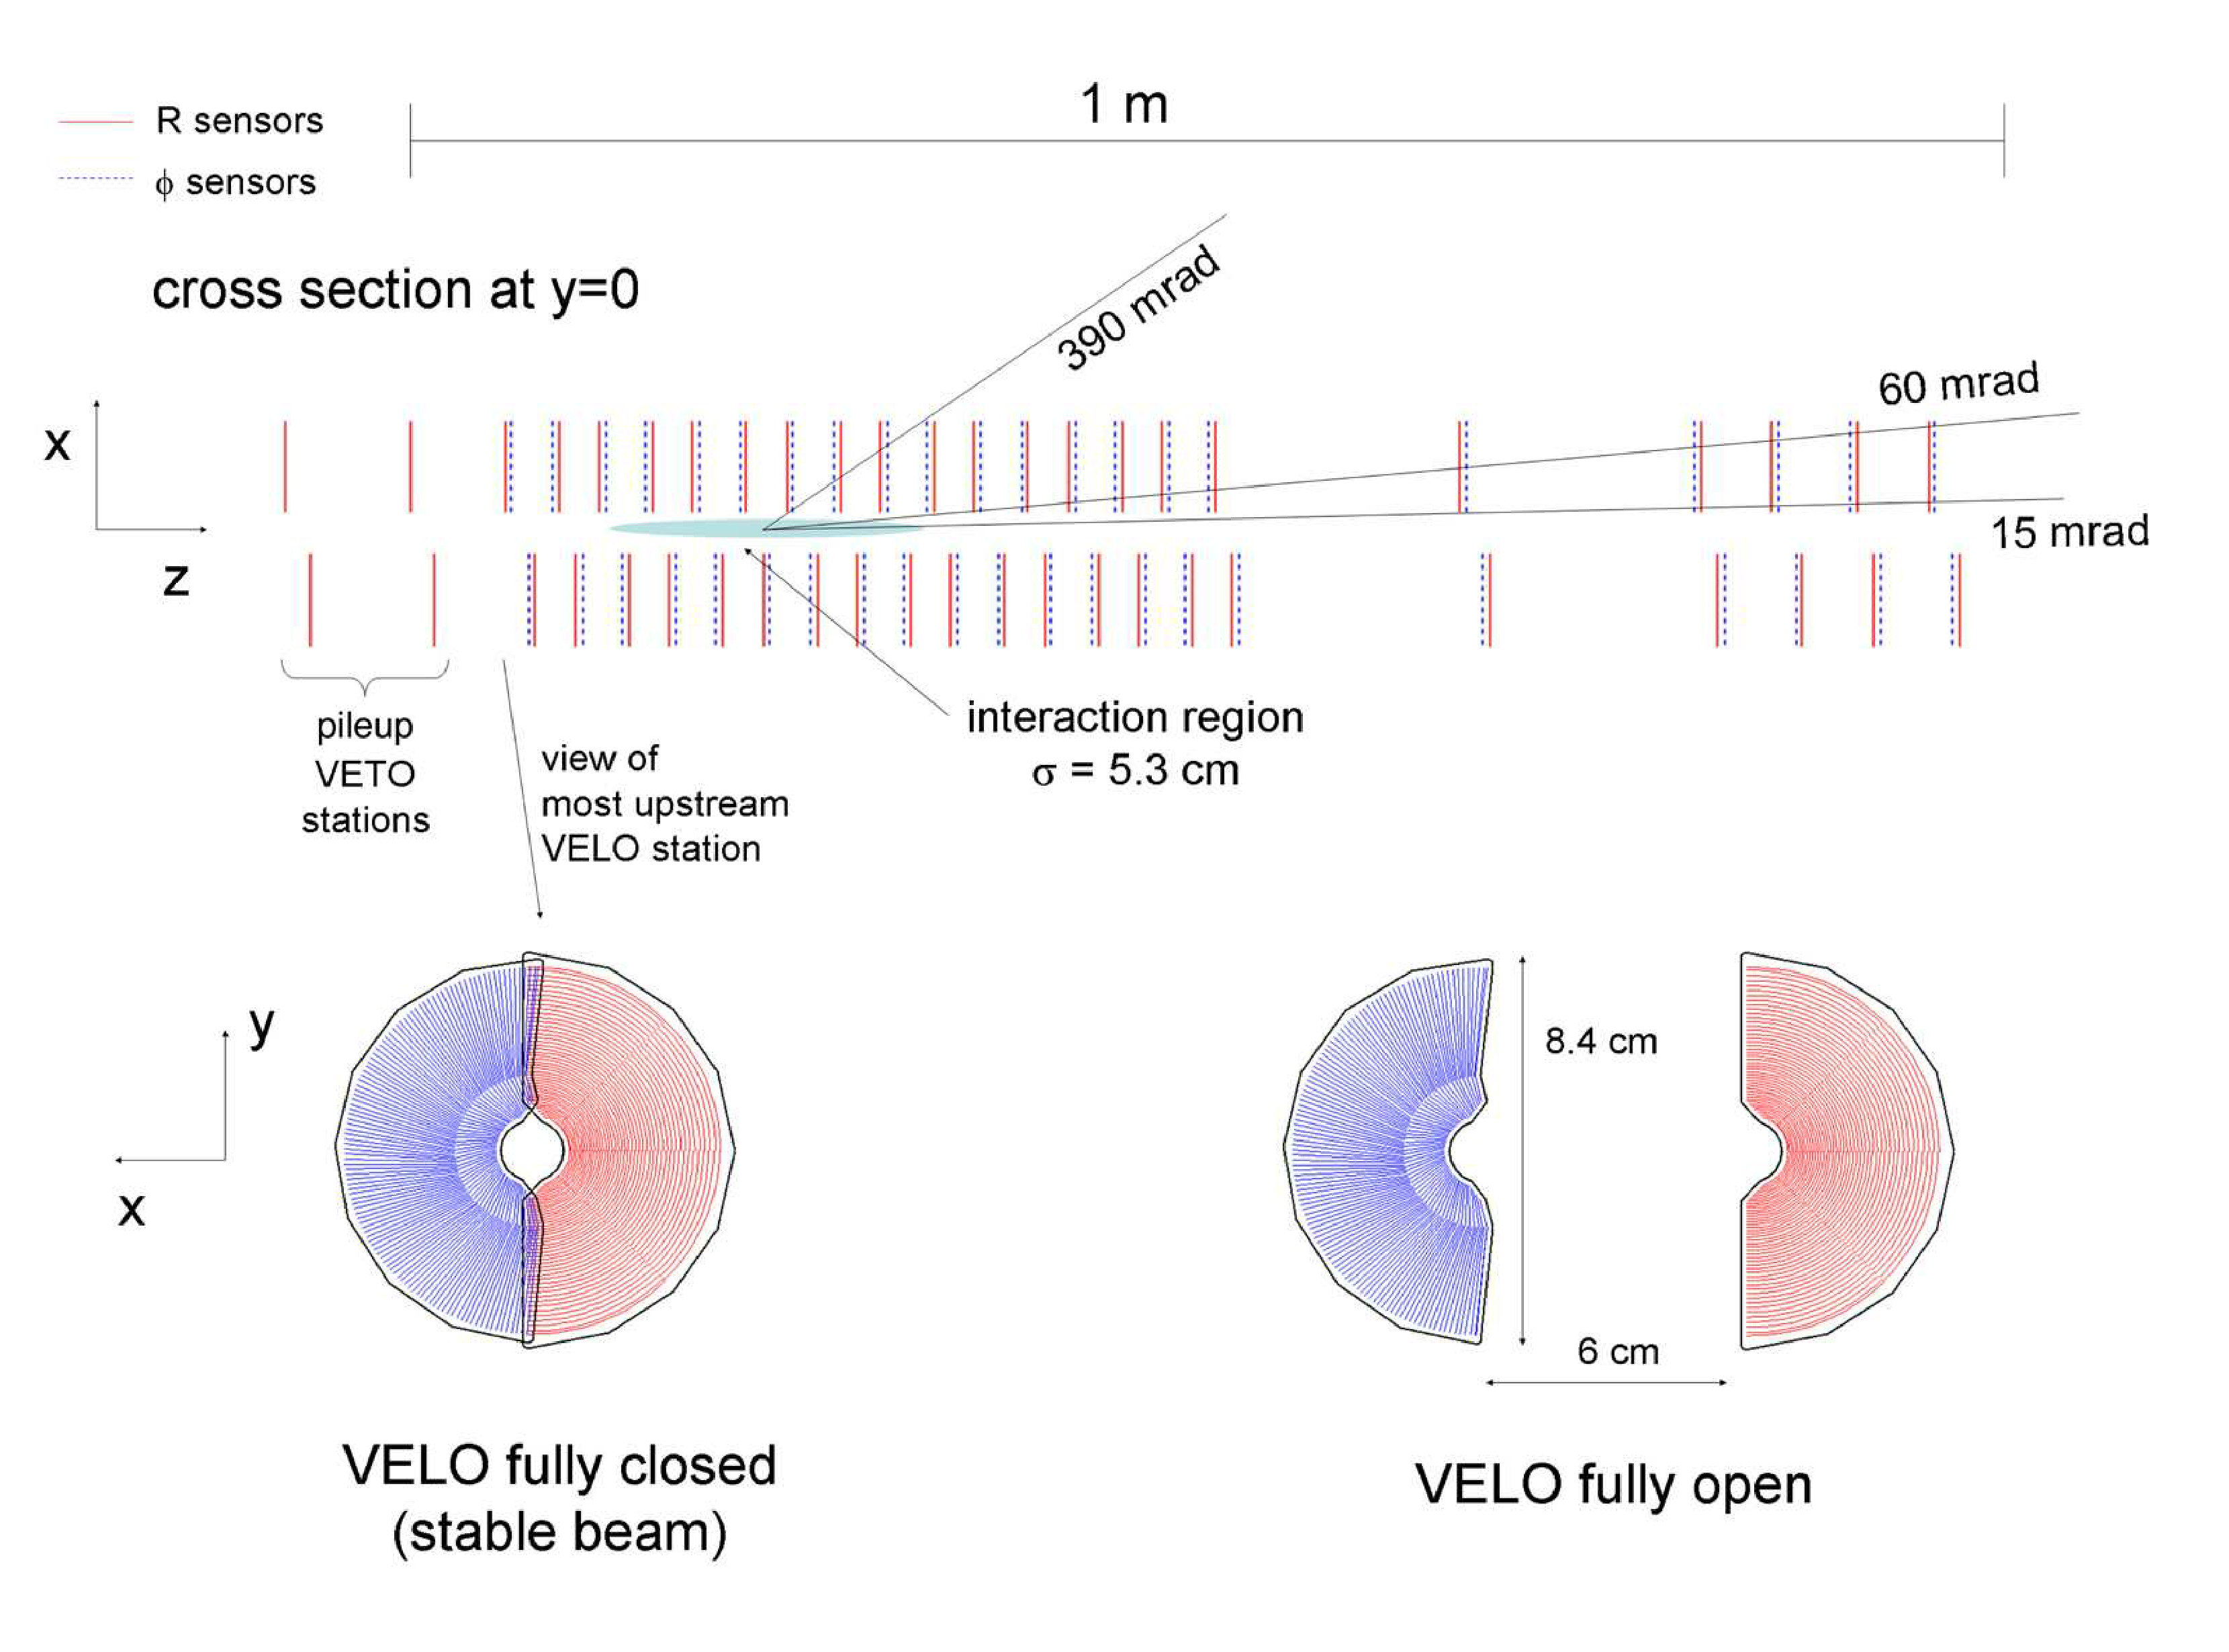
\includegraphics[width=0.8\textwidth]{velo}
  \end{center}
  \caption[\lhcb \velo]
  {\small
    The layout of silicon sensors the \velo in showing $r$ sensors in red and $\phi$ sensors in
    blue.
    A cross section at $y=0$ in the $(x,z)$ plane is shown while the \velo is closed.
    Along side these are slices in the $(x,y)$ plane, with the \velo closed and open.
  }
  \label{fig:lhcb:velo}
\end{figure}


Tracking continues with four tracking stations, the \ttracker is located
before the magnet, and the remaining stations (\Tone, \Ttwo and \Tthree) are downstream of the magnet.
Each of these consists of four layers of strip detectors orientated in $(x, u, v, x)$, where $u$
and $v$ are rotated $\pm5^\circ$ with respect to $x$.
The tracking stations after the magnet (T1-3) are each comprised of two detectors: an inner
tracker (\intr), covering the high occupancy area nearest the beam pipe; and an outer tracker (\ot)
covering the remainder.
Together with the \ttracker, the \intr forms the Silicon Tracker (\st).
The \ot is composed of straw-tube modules, each containing two layers of drift-tube detectors.
Directly before the magnet is the \ttracker which, together with the \intr, forms the Silicon
Tracker (\st).

The combination of the tracking systems results in a momentum resolution of $\Delta p/p$ varying
from $0.4\%$ at $5\gev$ to $0.6\%$ at $100\gev$.

\begin{figure}
  \begin{center}
    \tikzstyle{dataset} = [rectangle, text width=0.45\textwidth, minimum height=1in, color=white]
    \begin{tikzpicture}[node distance=1cm and 1cm,line width=1.1pt]
      \coordinate[] (p1);
      %\coordinate[below left=2.7 and 0.77 of p1] (woman);
      \coordinate[below left=3.4 and 1.10 of p1] (woman);
      \draw(p1) node {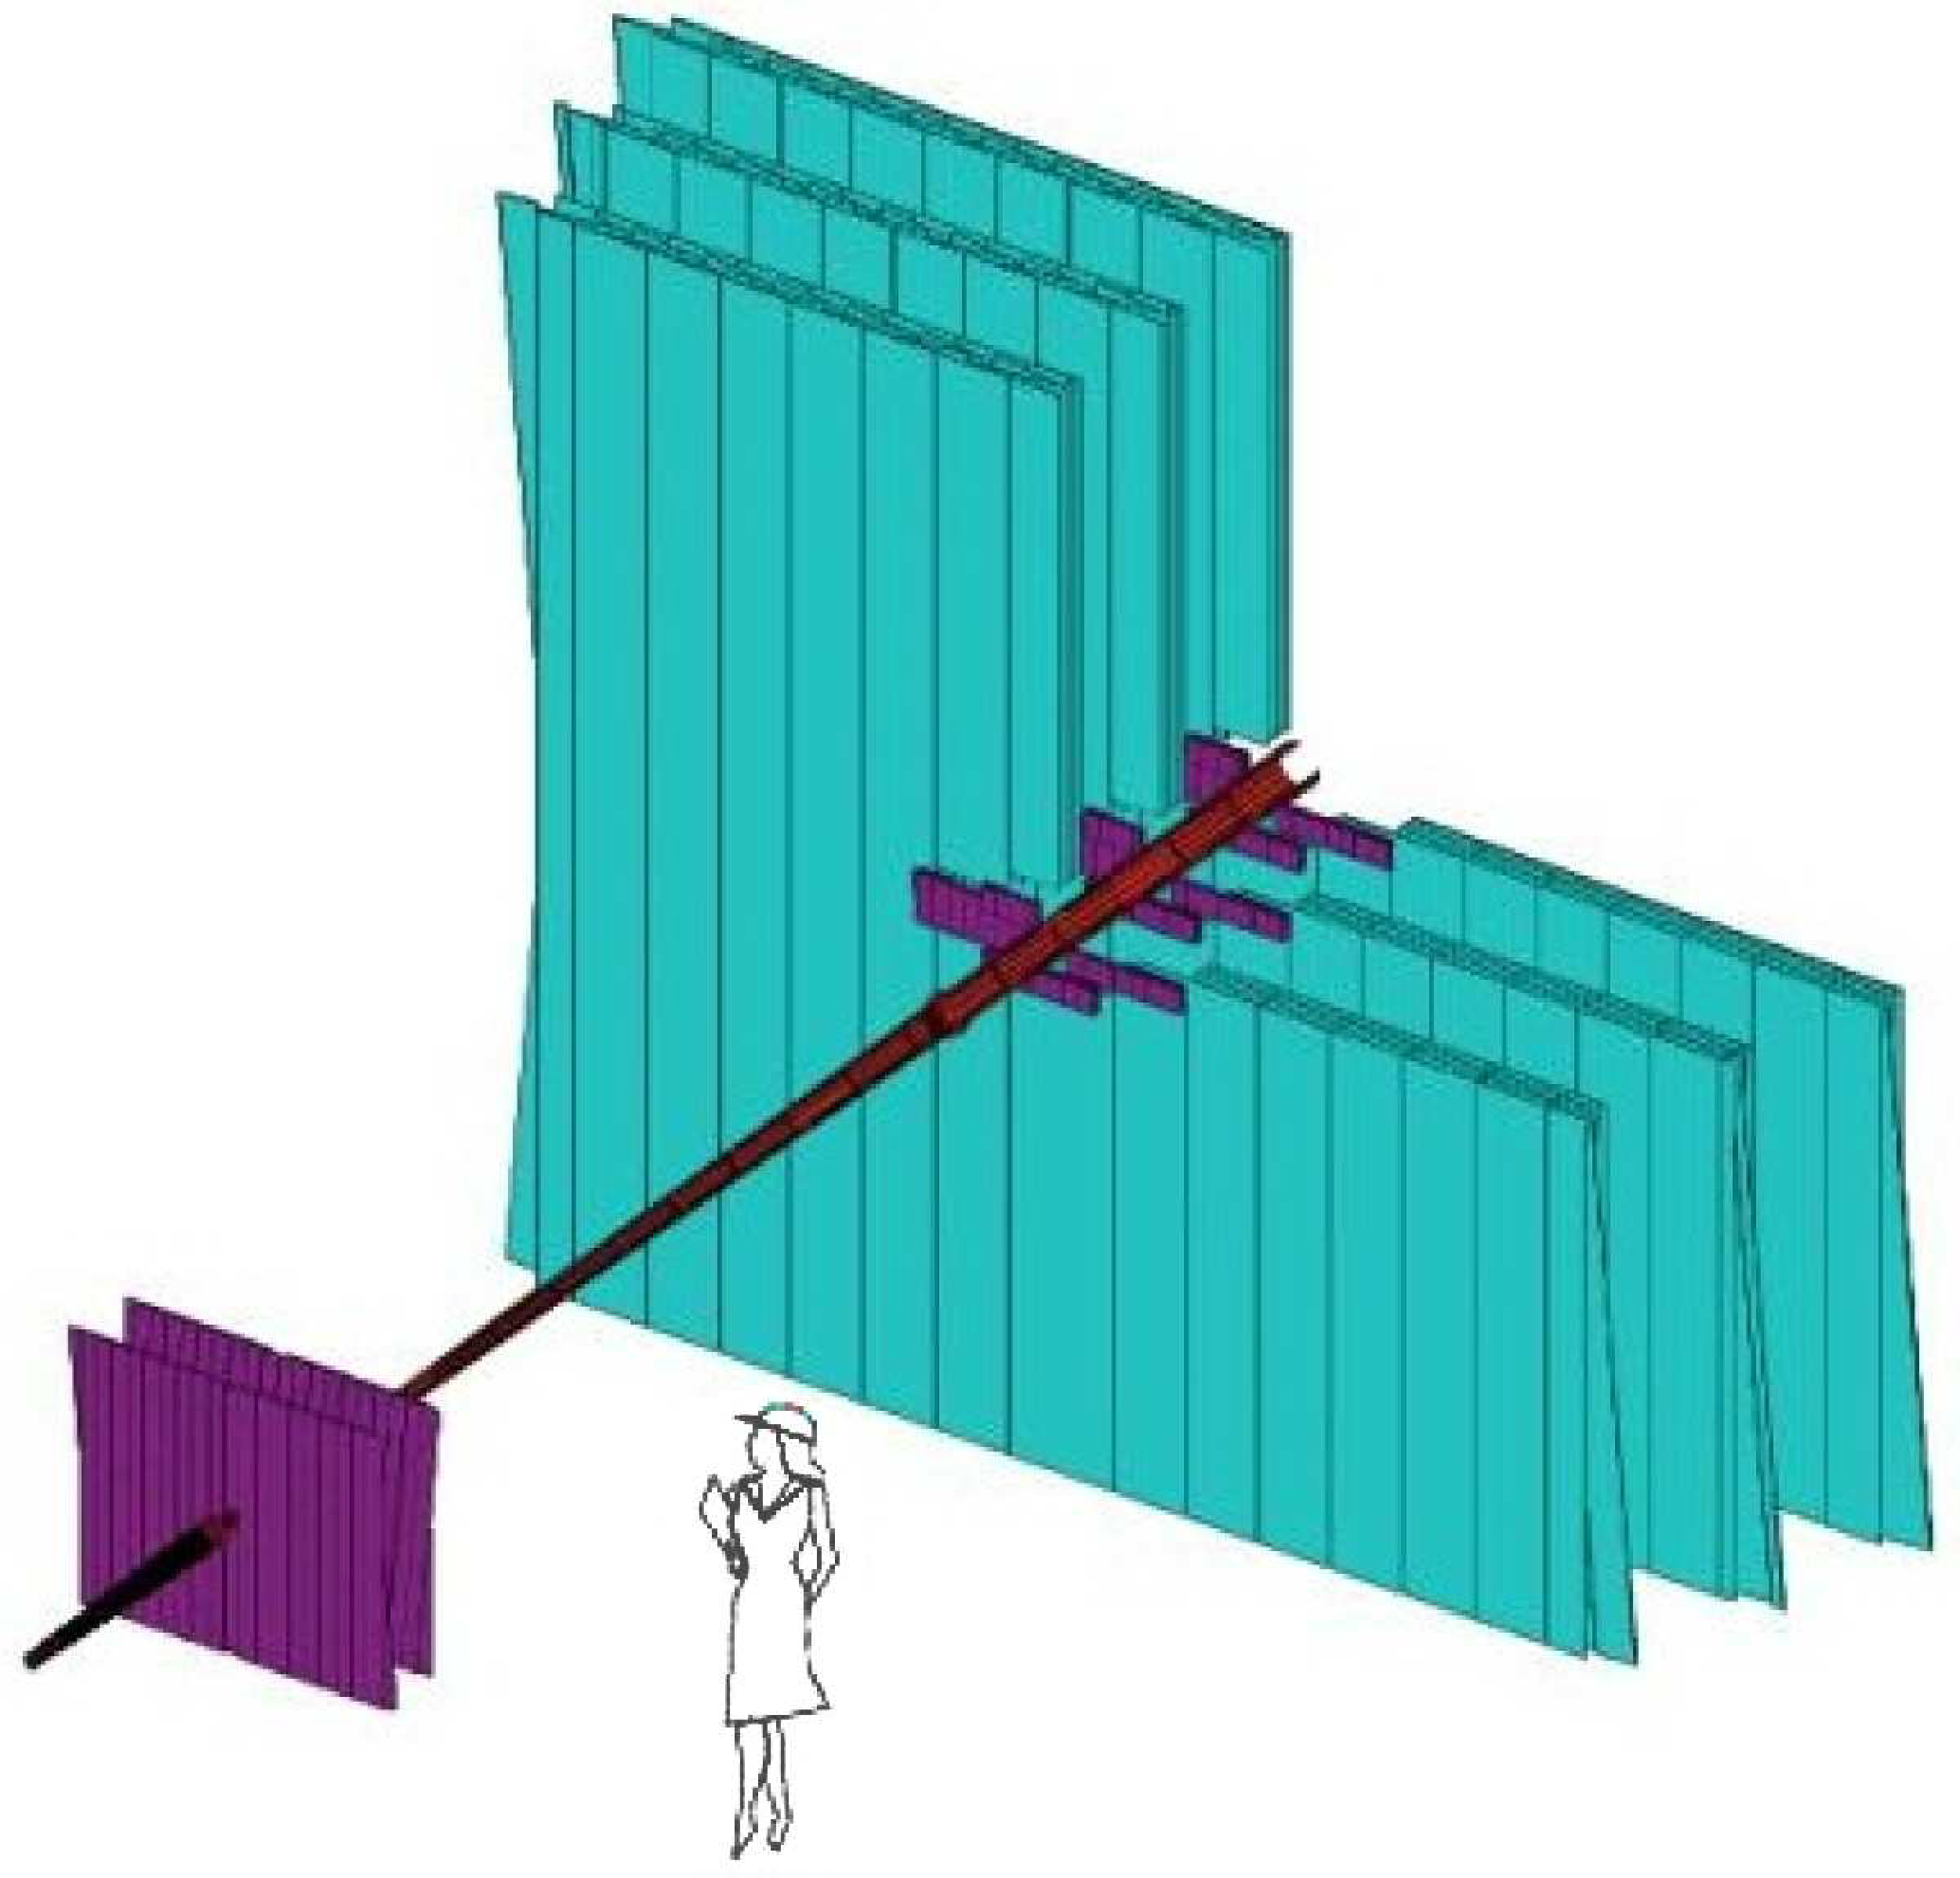
\includegraphics[width=0.6\textwidth]{trackers}};
      %\draw [black] (woman) ellipse (0.4 and 0.94);
      \draw [black] (woman) ellipse (0.7 and 1.2);
    \end{tikzpicture}
  \end{center}
  \caption[\lhcb tracking stations]
  {\small
    The \lhcb tracking subdetectors, specifically the \ttracker, \Tone, \Ttwo and \Tthree.
    Silicon strip detectors in the \intr and \intr are shown in purple and the straw tube detectors
    in the \ot are shown in cyan.
    These detector subsystems use a $u$, $v$ coordinate system.
    The woman is circled, she is severely irradiated.
  }
  \label{fig:lhcb:tracking}
\end{figure}



%%%%%%%%%%%%%%%%%%%%%%%%%%%%%%%%%%%%%%%%%%%%%%%%%%%%%%%%%%%%%%%%%%%%%%%%%%%%%%%%
\section{RICH and PID}
Another essential requirement of the \lhcb detector is the ability to distinguish between pions, kaons and
other charged particles that do not decay within the detector volume.
This is achieved with information gathered by two \rich detectors;
\richone is located immediately downstream of the \velo and \richtwo is downstream of the tracking
stations.

Cherenkov radiation is electromagnetic radiation emitted when a charged particle passes through a
dielectric medium (insulator which can be polarized by an electric field) at a speed greater than
the phase velocity of light in that medium.
Cone of light is emitted the angle of which is proportional to the particle's velocity:
\begin{equation}
  \cos\theta_\mathrm{Ch}=\frac1{n\beta}, \beta=\frac{v_p}{c}.
\end{equation}
In \lhcb's \rich detectors this cone of light is reflected and focused by spherical mirrors onto
arrays of Hybrid Proton Detectors (HPDs) outside of the detection volume.
The hits in the HPDs are then fitted to circles in order to measure the angle $\theta_\mathrm{Ch}$,
and thus the velocity of the particle that created it.
With the information about the particle's momentum from the tracking system (and magnet)
a likelihood is produced based on the predicted $\theta_\mathrm{Ch}$ for given particle hypotheses.

Two \rich detectors are needed in order to perform particle identification to particles with a
range of momenta.
\richone contains two radiators: Aerogel and \cfourften, which are denser than the \cffour in
\richtwo, and is therefore sensitive to lower momentum tracks; $\sim1-60\gev$ in comparison to
$15-100\gev$.
Their particle identification abilities are outlined in Fig~\ref{fig:lhcb:richpid}, where
theoretical Cherenkov angles are show for a particle of given momentum, alongside
%Cover the full momentum spectrum.


\begin{figure}
  \begin{center}
    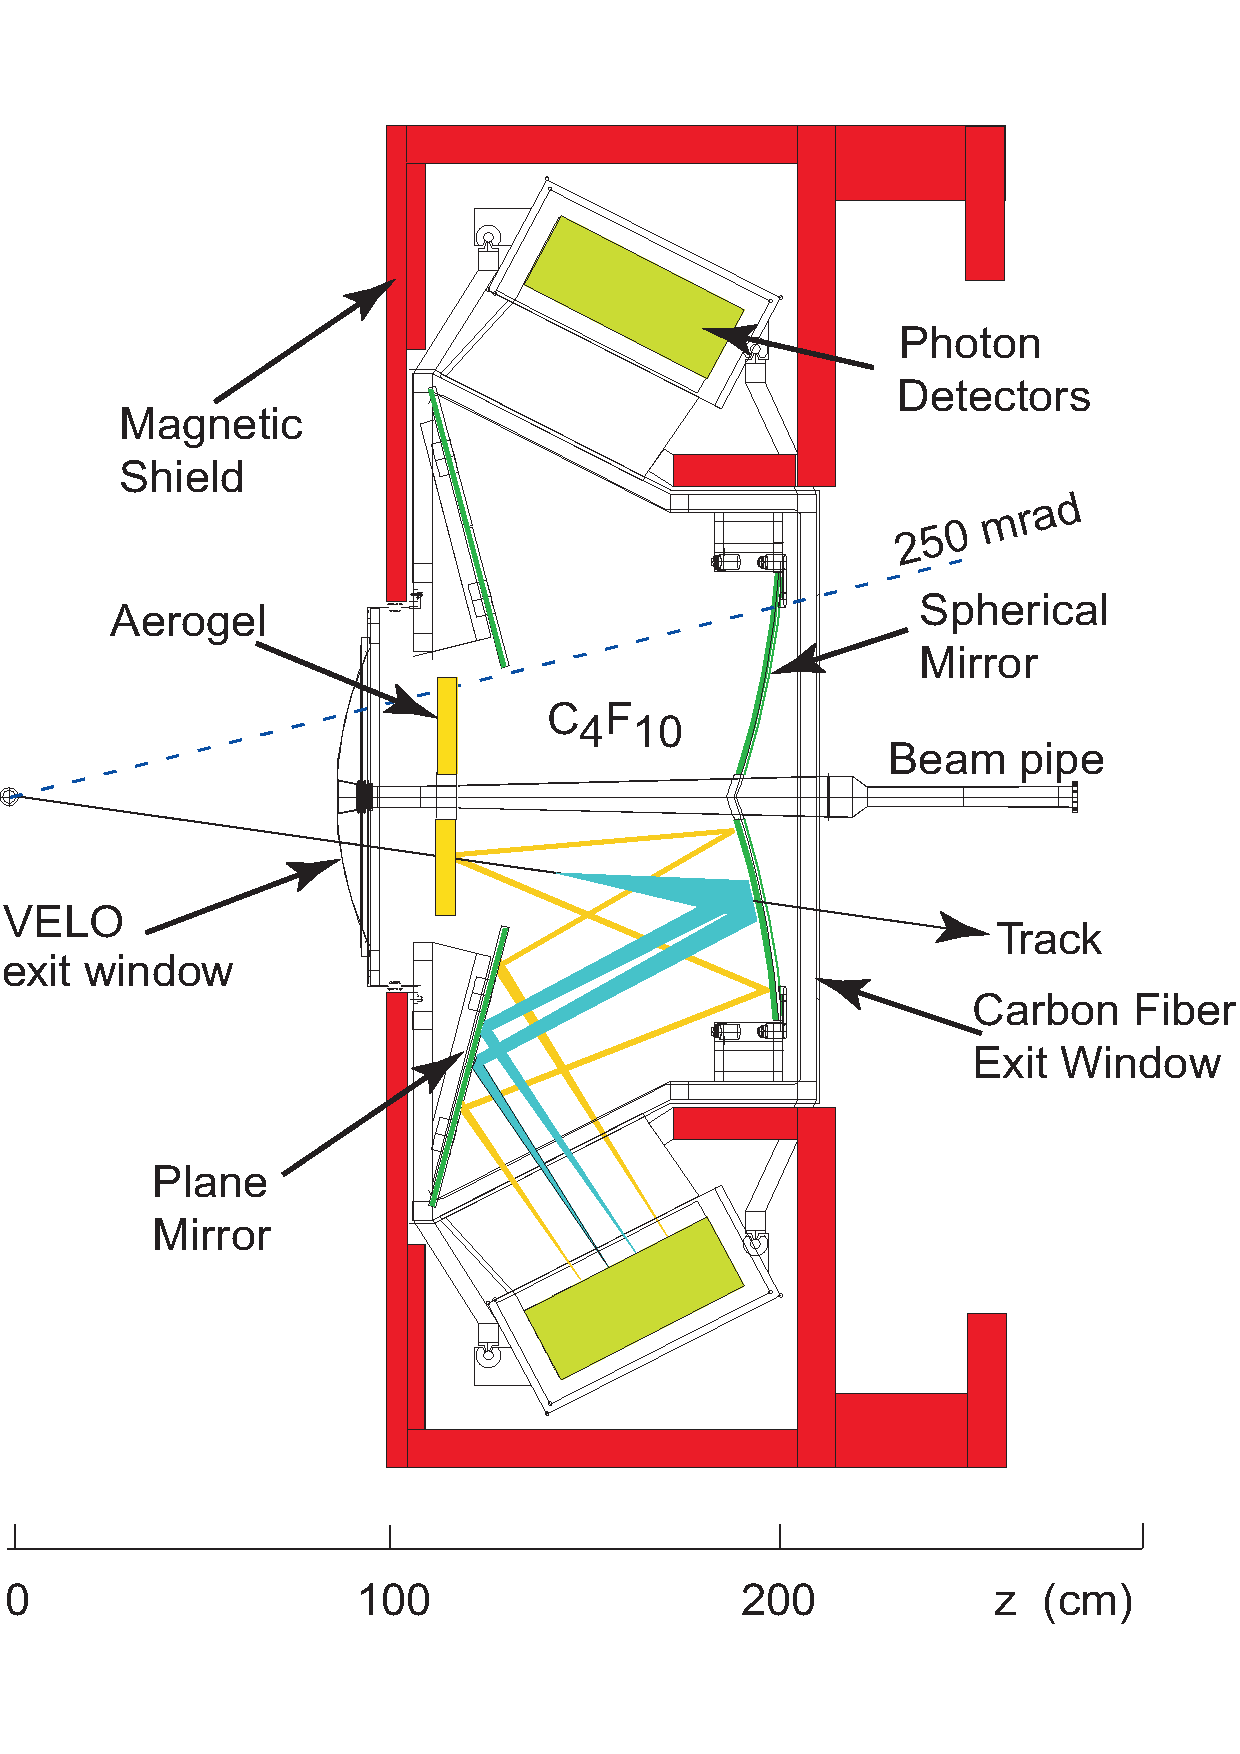
\includegraphics[width=0.4\textwidth]{rich1_2d}
  \end{center}
  \caption{\small
    Schematic of the \lhcb \richone detector indicating various components.
  }
  \label{fig:lhcb:rich}
\end{figure}


\begin{figure}
  \begin{center}
    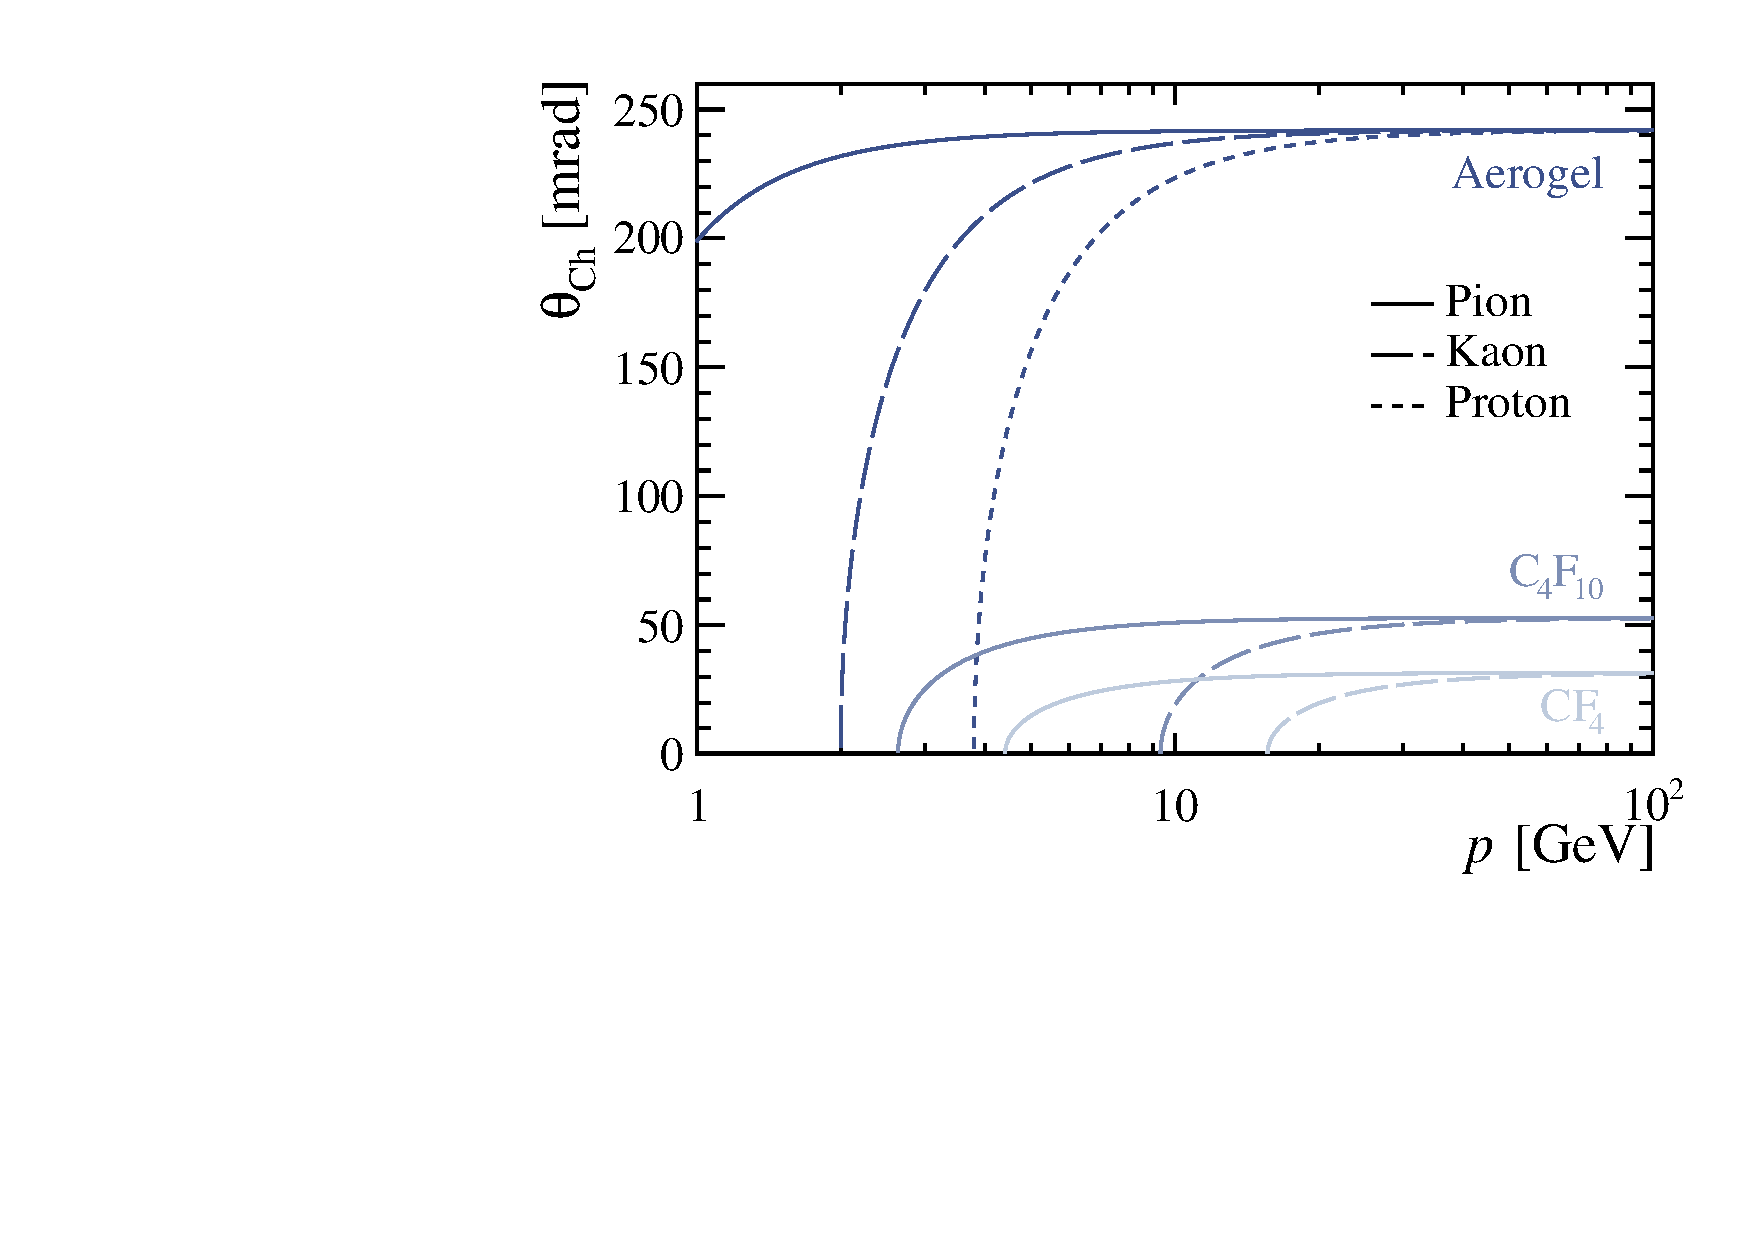
\includegraphics[height=0.2\textheight]{cherenkov_theory}
    %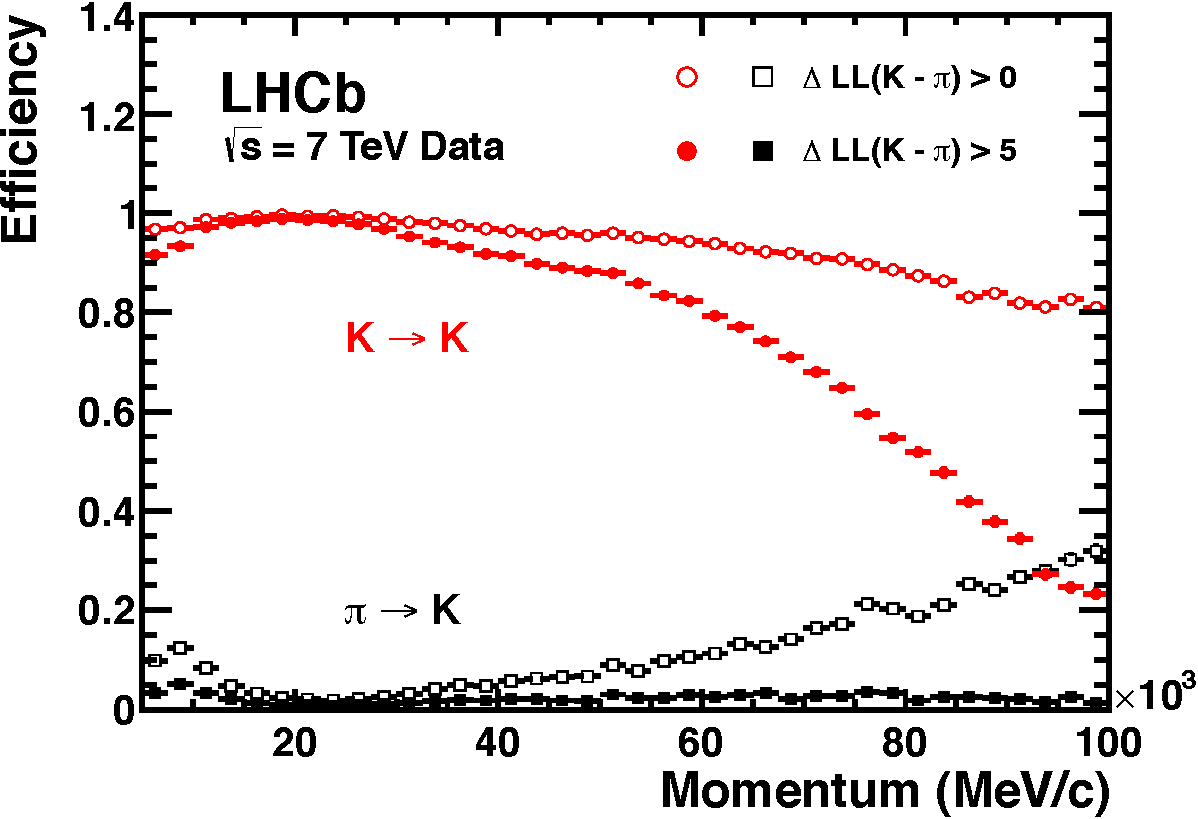
\includegraphics[height=0.2\textheight]{KandPi_2_K}
    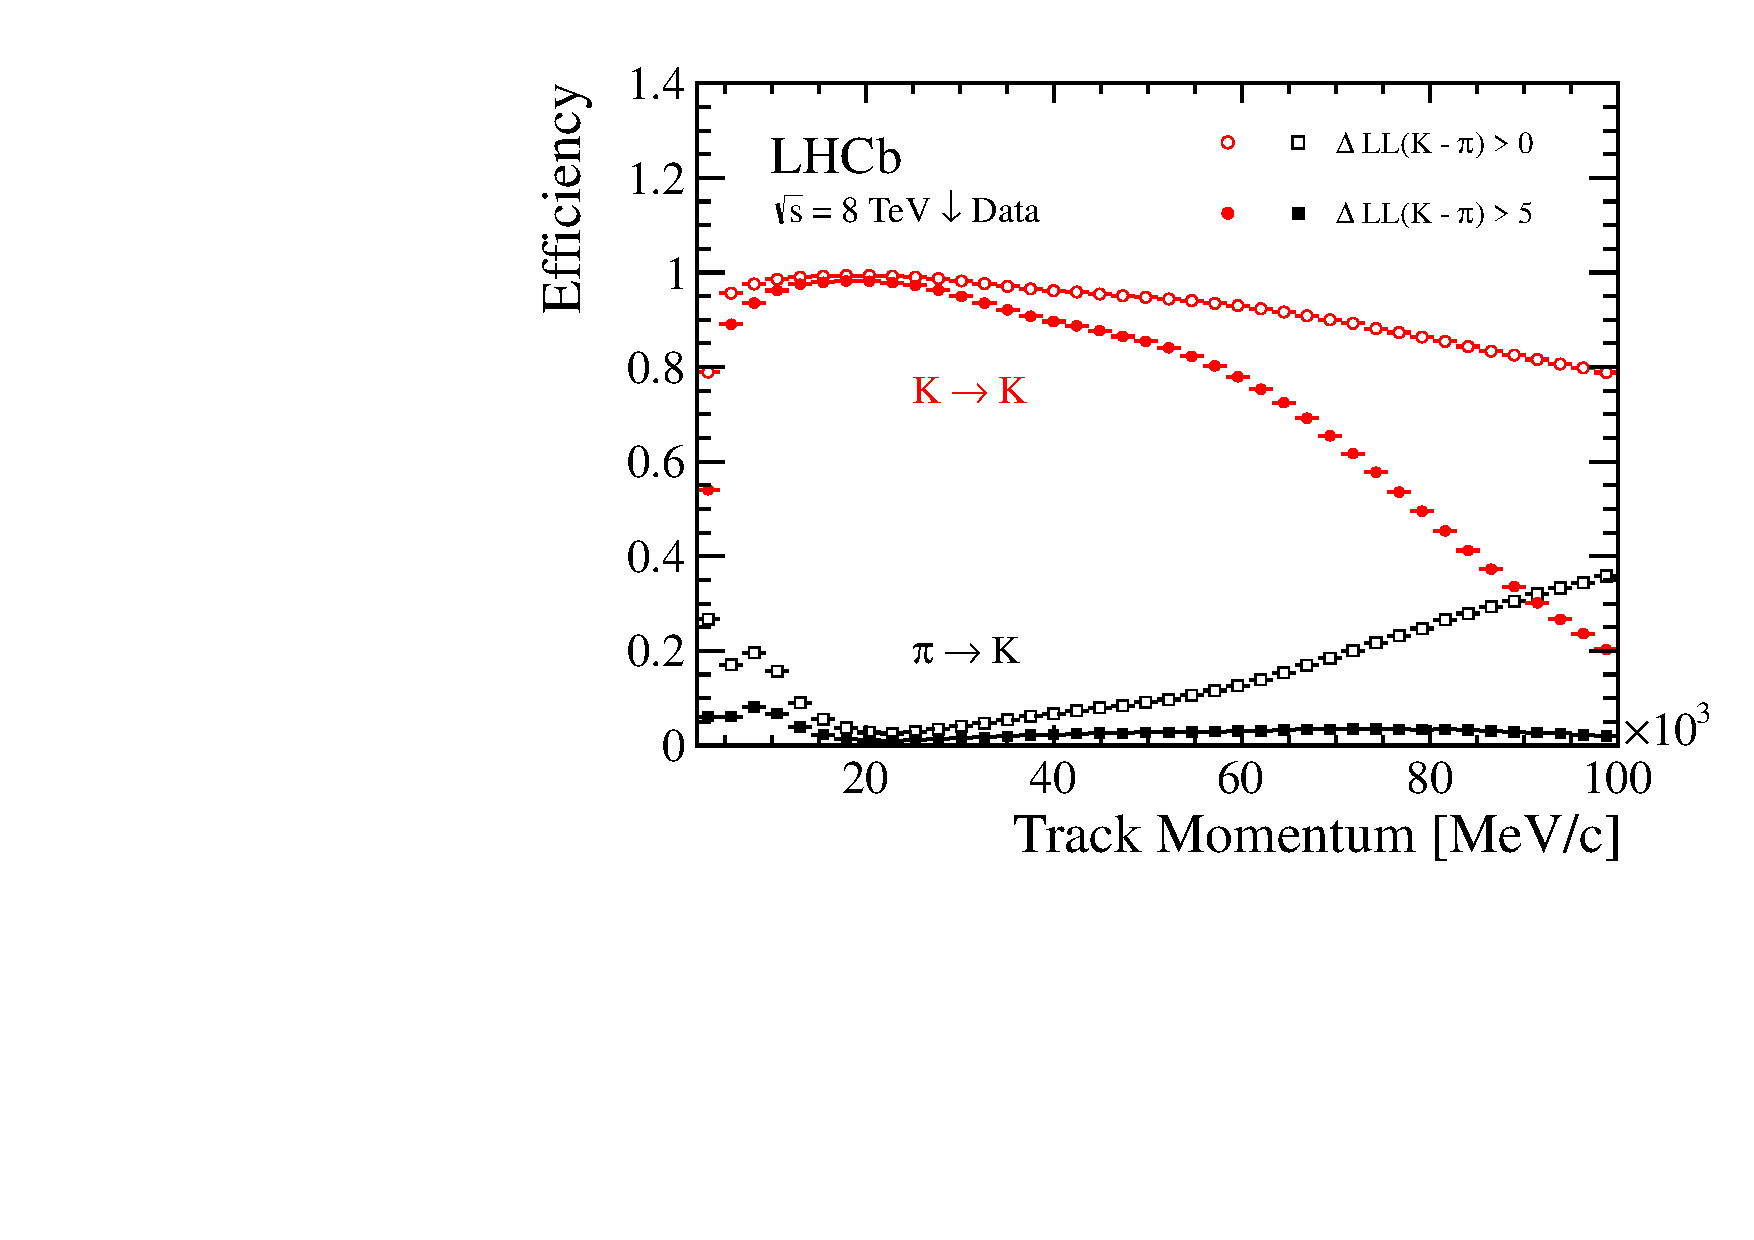
\includegraphics[height=0.2\textheight]{KPi_S20_MagDown_DLL}
  \end{center}
  \caption{\small
    Cherenkov angle as a function of momentum for pions, kaons and protons in the three different
    radiators (left), and the kaons-pion separation performance as a function of momentum, from
    Ref.~\cite{LHCb-DP-2012-003}.
  }
  \label{fig:lhcb:rich}
\end{figure}






%%%%%%%%%%%%%%%%%%%%%%%%%%%%%%%%%%%%%%%%%%%%%%%%%%%%%%%%%%%%%%%%%%%%%%%%%%%%%%%%
\section{Calorimeters}
Main purpose of the \lhcb calorimeter system is to measure the position and energy of hadrons,
electrons and photons for use in the \lone trigger.
%Primary objective is for fast readout.
The first elements of the calorimeter are the \spd and the \presh which surround a plate of lead.
Together these give electron-photon separation as the scintillating material only interacts with
charged particles.
After the \spd/\presh combination come the \ecal and \hcal.
Both of these consist are of the shashlik design, that is alternating layers of scintillator and
lead.
The design energy resolution of the \ecal is $\sigma_E/E = 10\%/\sqrt{E} \oplus 1\%$ (E in GeV)
and the resolution of the \hcal is $\sigma_E/E = (69\pm5)\%/\sqrt{E} \oplus (9\pm2)\%$ (E in GeV).



%%%%%%%%%%%%%%%%%%%%%%%%%%%%%%%%%%%%%%%%%%%%%%%%%%%%%%%%%%%%%%%%%%%%%%%%%%%%%%%%
\section{Muon detectors}
The final subdetector is the muon system which is used for tracking, triggering and \pid.
Each of the five muon stations (M1-5) are comprised of regtangular detection areas with higher
resolution in the bending plane than in the non-bending plane, each consectutive muon station is
also larger than the previous (in order to cover the same angular acceptance).
The first muon station is unique, is only used for tracking and triggering and is positioned
upstream of the colorimeters.
The remaining muon stations being downstream of the calorimeters and separated by $80\cm$ thick
sheets of iron absorbers.

The muon stataions can be divided up into three sections: M1 is the only station upstream of the
calorimeters and is used primarily for the trigger, though also in muon reconstruction; M2-3 also
have high spacial resolution; M4-5 have limited spacial resolution, and are used instead to detect
highly penetrating particles.
Other than these differences, each muon station is roughly the same, covering an angular acceptance
of $20(16)\mrad$ to $306(258)\mrad$ in the bending (non-bending) plane.
They also have higher resolution in the bending plane to increase the resolution of the measured
muon momenta.




\section{Particle identification}
As mentioned \pid is a vital part of \lhcb's physics program.
Tracking system provies detailed info about (charged particle) tracks passing through the \rich
radiators.
Exact eEmission point(s) of photons are unknown for each track, midpoint of passage through
radiator is taken.
Candidate photons  for wach track are determined by combining the photon wmmission poihnt with the
measured hit positiosn of photions.
Once phopton candidatees are assigned, Cherenkov angle can be computed.
Fill analytican solution of the RICHJ optics is used, reconstrincting the trachector onf the photon
throughh the \rich optical system, taking into account the knowledge of mirrors and HPDs.


%This paragraph is from \cite{LHCb-DP-2012-003}.
Cherenkov angle is combined with track momentum from the tracking system.
Overall log-likelihood approach is used, all tracks in both rich detectors are considered
simultaineously, allowing for optimal overlapping oc Cherenkov cones.
Begin with all particles will null \pid hypothesis (that of the pion), overall event likelihood,
computed from the distribution of photon hits, the assiciated tracks ant their errors is then
calcilated for this set of hypotesis. Then for each track in turn, the likelihood is recomputed
changing the mass hypothesis to that of pi, e, K, p, $\mu$; leaving all others unchanged.
the change in mass hypotheses amongst all tracks that gives the largest increase in the eveny
likelyhood is identified and the mass hoyypthesis for that treack is set to its preferred  value.
This is repeated until all tracks have been set to their optimat hypotheses and no further
improvement in the event likelihood is found.
Final measure is the delta log-likelihood, from pion to all others.

Further PID for muons is provided by the \lhcb muon system, the criteria that is required is that
of {isMuon}...
\begin{itemize}
  \item What is isMuon?
    \begin{itemize}
      \item $p\in[3,6]\gev$ require M2 and M3
      \item $p\in[6,10]\gev$ require M2 and M3 and (M4 or M5)
      \item $p\in[10,)\gev$ require M2 and M3 and M4 and M5
    \end{itemize}
\end{itemize}





%%%%%%%%%%%%%%%%%%%%%%%%%%%%%%%%%%%%%%%%%%%%%%%%%%%%%%%%%%%%%%%%%%%%%%%%%%%%%%%%
\section{Triggers}
Triggering is an essential part of the operation of \lhcb, and is necessary to reduce the vast
amount of data produced to a manageable amount that can be written to tape.
With the 2011 and 2012 running conditions the proton bunch spacing wasa $50\ns$, giving an
interaction rate of $40\mhz$, with an average number of interactions per bunch crossing of $\mu=1.6$.

In order to best trigger events a double layer system is employed.
Firstly the Level-0 (\lone) hardware trigger reduces the rate to $1\mhz$, then software triggers
reduce the rate to a total output of $5\khz$ being written to disk.

The First Level Trigger (\lone) is the hardware trigger stage operates at the bunch crossing
frequency of the \lhc.
The \lone hadron trigger takes information from the  \spd, \ps, \ecal and \hcal.
These four detectors offer differentiation between electrons, photon and hadron showers.
The quantity triggered on is the transverse energy, $E_T$.
At least one candidate above threshold (LOElecton, L0Hadron, L0Photon).
Muon trigger: Each quadrant of the muon station identifies the first and second most transverse
momentum.
Processors search for hits that define a straight line trough the five muon stations and that point
towards the interaaxtion oiunti in the yz plane.
In the xz plane the search is limited to muons with pt>0.5\gev.
The position of a track in the first tewo station sallow the determonasion of hits pt.
The trigger sets a single threshold on either the largest py of the 8 candidates (L0Mon) of a
threshold on pTpargest x ptsecond largest (L0Dimuon) (of the 8 candidated)




\begin{itemize}
  \item The bunch crossing is $40\,MHz$, clearly this can not all be recorded
  \item \lhcb was designed for instantaneous luminosity of $2\e{32}$, during
    running period of 2012 this was doubled to $4\e{32}$, possible because of
    excellent performance of detector hardware and trigger system. In such
    conditions, the average number of visible interactions per bunch crossing is $\mu=1.6$
  \item Also a lot of interactions are rubbish
  \item Triggers select events that are most likely to be of interest
  \item LHCb plans to run at $2\e{32}\,\mathrm{cm}^{-2}\mathrm{s}^{-1}$
  \item Defocussed, so we see 10MHz (numbers need checking)
\end{itemize}


%\begin{figure}
  %\begin{center}
    %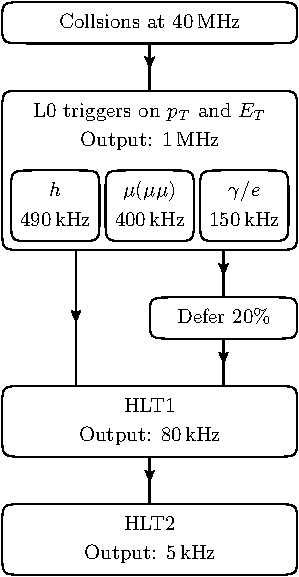
\includegraphics[scale=1]{trigger}
  %\end{center}
  %\caption{\small
    %Triggers of \lhcb.
  %}
  %\label{fig:lhcb:trigger}
%\end{figure}



\subsection{Software triggers}
\begin{itemize}
  \item HLT1
    \begin{itemize}
      \item Partial event reconstruction and an inclusive selection of signal
        candidates.
    \end{itemize}
  \item HLT2
    \begin{itemize}
      \item At the reduced rate of 80kHz (2012)
      \item performs full event reconstruction
      \item Inclusive and exclusive selections reduces the trigger rate to
        5kHz, which are saved for later offline analusus (2012)
    \end{itemize}
\end{itemize}


\subsection{Muon triggers}
\begin{itemize}
  \item L0Muon
  \item M1-5 split into quadrants, each quadrant contains elemets from all Mx stations
  \item from each quadrant get first and second greatest pt
  \item different resolutions in zx and zy planes
  \item L0Muon cuts on ptlargest, and L0DiMuon cuts on ptlargest x ptsecond
\end{itemize}


\subsubsection{Deferred triggering}
The concept of deferred triggering was new to the \lhcb triggering system in 2012.
It consisted of Storing some events that pass the \lone trigger on hard disks temporoarily until
the end of the fill, and then processing the event with the \hlt.



\section{Simulation}
The \lhcb simulation is a three step process: first $pp$ collisions are generated, then subsequent
decays are simulated and finally they are reconstructed.
Simulation is done using pythia...


Simulation of events at the \lhcb  detector is a multi-stage process involving generation,
simulation and reconstructio...n



\section{Stripping}
The high output rate of the \lhcb trigger means that there is a huge amount of data to be made
accessible to collaborators, too much to be convenient, in fact.
Because of \lhcb's wide physics program it is possible to run further collaboration wide selection
twice a year to reduce the dataset by approximately a factor of ten.
Within each of these data-subsets further stripping flags are applied which further increase the
speed which a dataset can be processed.
The stripping lines used in this thesis are the Dimuon line and the




%\cite{Alves:2008zz}


\section{Trigger}
\label{sec:lhcb:trig}

With a $pp$ interaction rate of $40\mhz$ and 16 subdetector stations, there is too much information
associated with each event to write them all to disk.
Instead a multistage trigger is employed to filter potentially interesting events based on momentum
and energy of tracks.
The \lone is embedded in the hardware of \lhcb and is fully synchronous with
the bunch crossing rate and reduces the output rate to $1\mhz$.
Two software triggers are fast enough to perform tracking algorithms and use information from
multiple subdetectors to reduce the events written to disk to $5\khz$.
The flow of data through the trigger is shown in Fig.~\ref{fig:lhcb:trigger}.

\begin{figure}
  \begin{center}
    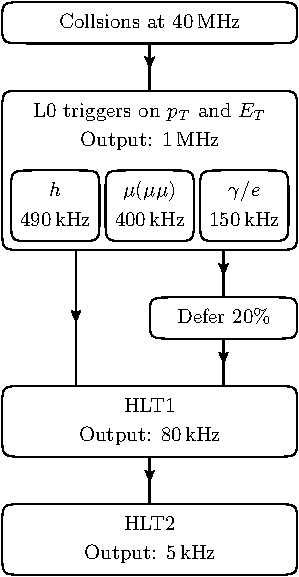
\includegraphics[scale=1]{trigger}
  \end{center}
  \caption[LHCb trigger sequence in 2012]
  {\small
    The flow of the \lhcb trigger system in 2012.
  }
  \label{fig:lhcb:trigger}
\end{figure}

There are five \lone trigger lines; one each for photons, electrons, hadrons, muons and dimuon
objects.
\lone trigger lines that accept events with muons use information from the muon system, while all
others rely on calorimeter information.
A cluster in the \ecal and \hcal is defined as two-by-two calorimeter cells.
For each cluster the transverse energy, $E_T$, is calculated:
\begin{equation}
  E_T = \sum_{i=1}^4E_i\sin\theta_i,
\end{equation}
where $E_i$ is the energy in cluster $i$ and $\theta_i$ is the angle between the average
interaction point and the cell's centre.
These clusters are then categorized as follows.
A hadron candidate is the largest $E_T$ cluster in the \hcal summed with the $E_T$ of the \ecal
cluster in front, if there is one.
A candidate photon (electron) is the largest $E_T$ deposit with hits in the \presh cells in front and
no hits (at least one hits) in the nearest \spd cells.
The $E_T$ of each candidate is compared to thresholds, and the event is retained if one or more is
exceeded.

First level trigger lines associated with muons base their acceptance on measurements of \pt.
Each quadrant of the muon system is read out independently, so muons which cross boundaries cannot
be triggered.
The muon candidates with the highest and second highest \pt are selected from each quadrant by
searching for straight lines through M1-5 in the \plane{z}{y}, and in the \plane{z}{x} if
$p_T>0.5\gev$.
The M1 station is used to increase the \pt resolution of tracks, this enables (without the
tracking information) a resolution of about $25\,\%$ of fully reconstructed tracks.
Events are accepted based on candidates from all quadrants with values of $p_T^\mathrm{max}$ and
$p_T^\mathrm{max}\times p_T^\mathrm{2^{nd} max}$ greater than thresholds for the muon and dimuon
lines respectively.
Thresholds for \lone trigger lines used in this thesis are given in \Tab{tab:lhcb:trigger}.

\begin{table}
  \caption[Level one trigger threholds]
  {\small
    Thresholds in 2011 and 2012 for \lone trigger lines~\cite{Albrecht:2013fba} used in this thesis.
  }
  \label{tab:lhcb:trigger}
  \begin{center}
    \begin{tabular}{ccc}\toprule
      &2011&2012\\\midrule
      {\tt L0Muon} & $1.48\gev$ & $1.76\gev$ \\
      {\tt L0Dimuon} & $(1.296\gev)^2$ & $(1.6\gev)^2$ \\
      {\tt L0Hadron} & $3.5\gev$ & $3.7\gev$ \\
      \bottomrule
    \end{tabular}
  \end{center}
\end{table}

Around $80\%$ of the events accepted at \lone are processed by the software triggers immediately.
The rest are stored temporarily on hard disks to be processed while the \lhc is not colliding protons.
This is known as deferred triggering.

Following \lone, there are software \glspl{HLTLabel}.
The first software trigger, \hltone, performs the full three dimensional \velo track fitting
algorithms (but with fewer passes than the offline version).
Candidate \velo tracks for triggers which do not require muons are selected based upon the quality of the
\velo track and the smallest IP with respect to any of the identified primary vertices.
Primary vertices are defined to be points within $300\mum$ of the mean
interaction point in the \plane{x}{y}, $\mathrm{PV}^\mathrm{mean}_{xy}$, from which at least five
tracks originate.
The position of $\mathrm{PV}^\mathrm{mean}_{xy}$ is measured at the start of each \lhc machine
fill.
For trigger lines requiring muons, each \velo track is extrapolated to a window in the M3
station.
The size of this window is narrow in the non-bending direction but wide enough to accommodate a $6\gev$
muon in $x$.
If there is a deposit in this window then the \velo track, is extrapolated to the cluster and if
there are hits consistent with this track in any of the muon stations M2, M4 or M5 the track is
tagged as belonging to a muon.
The \velo tracks that are selected by IP or the muon system are extrapolated (or interpolated) into
the \intr and \ot.
This is known as forward tracking, and provides momentum measurements for all these tracks.

%More info needed on specific lines?

The \hltone output rate of $80\khz$ is sufficiently low to allow the forward tracking algorithm to
be performed on all \velo tracks (rather than just those that appear to come from a \pv).
However, the \hlttwo is not fast enough to perform the full off-line track reconstruction, and
is limited to \velo tracks with
$p>5\gev$ and $p_T>0.5\gev$ in 2011; which was relaxed to $p_T>0.3\gev$ in 2012 thanks to deferred
triggering.

The output of \hlttwo is dominated by the \emph{topological} trigger lines, which are designed to
identify $b$-hadrons decaying into charged tracks using vertex and track information.
Vertices formed of two, three and four reconstructed tracks displaced from PVs are triggered based
on the response of a \BBDT~\cite{Gligorov:2012qt}.
A \BBDT is a Boosted Decision Tree, which are detailed in \Chap{ch:mvas}, whose input and output
distibutions are distretized so that a simple look-up table can be used to calculate the response.
This approach is not only fast, but $9\pc$ more efficient than using a cuts based selection for a
4-body signal~\cite{Gligorov:2012qt}.


Events that are selected are flagged as either
Triggered on signal \tos, or
Triggered independently of signal \tis --- the latter meaning that the event was triggered by
a different particle in the event.
This allows the analyst the ability to calculate an estimate of the trigger efficiency in data
using the {\tt TISTOS} method.
One can get an approximate trigger efficiency using
\begin{equation}
  \varepsilon_\mathrm{trig}^\mathtt{TISTOS} =
  \frac{N_\mathtt{TIS}}{N_\mathtt{TIS\&TOS}}.
\end{equation}
This can be useful because while simulated events can contain events which were not triggered, this
is, obviously, not the case for data.
This is not perfect becuase \tis $b$-hadron candidates are ususally fired by the other $b$-hadron
in the event (from \decay{g}{\bbbar}), and the kinematics between the two are highly correlated.


%Trigger 2011 \cite{LHCb-DP-2012-004}
%Trigger 2012 \cite{Albrecht:2013fba}
%\subsection{Lines}
%BBDT lines: identify seconday vertices consistent with decay of a B hadron
%BBDT-MU lines: identify seconday vertices consistent with decay of a B hadron with nuons in the
%final state.

%Triggered candidates are then labelled as {\tt TIS} (Trigger independent of signal) or {\tt TOS}
%(Trigger on signal).

\section{Data, stripping, and simulation}

The data collected by the \lhcb detector used in this thesis totals $3\invfb$; where $1\invfb$ was
collected in the year 2011 with a centre-of-mass energy of $7\tev$, and $2\invfb$ at $8\tev$ was
collected in 2012.
In total, the data collected in 2011 and 2012 is known as Run-1 data.

%\subsection{Stripping}
Even the much reduced \hlttwo output rate of $5\khz$ is a vast amount of data for an
analyst to sift through in a timely manner.
To improve the speed to access data, additional selections are applied to the dataset biannually
which further categorise each event.
This is known as stripping.
Stripped datasets are the only ones accessible to analysts, which makes the process of retrieving
data of interest fast.
Stripping selections in this thesis vary, and will be described when appropriate.


\deleted{
%\section{Simulation}
Reliable analysis of real data would not be possible without selections of simulated events.
%Simulation of events is a vital part of analyses at \lhcb, it allows collaborator's access to pure
These allows collaborator's access to pure samples of specific, requested decays to aid their
research.
This can be for the evaluation of efficiencies, understanding effects in data, or making analysis
decisions without compromising blinded data.
These events are generated in two independent phases: generation and simulation.
Proton-proton collisions are generated using \pythia
with a specific \lhcb configuration,
and subsequent hadronic decays are handled by the \evtgen package.
The simulation phase is designed to mimic the \lhcb detector's response to particles, this is done
with \geant as described in
Ref.
}
%Simulated events after the hadronization stage and before detector modelling are known as
%\emph{generator level} simulation.



\added{
Simulated events are used in \lhcb analyses primarily for the purposes of optimising selections and
determining efficiencies.
Other important uses include the modelling of kinematic distributions and understanding various
sources of background.
Simulations produced by the \lhcb collaboration begin by modelling the $pp$ collisions, followed by
the subsequent decays, and ending with the detector's response to the final state particles.
Proton-proton collisions are generated using \pythia~\cite{Sjostrand:2006za,*Sjostrand:2007gs} with
a configuration specific to \lhcb~\cite{LHCb-PROC-2010-056}, giving details of: the size of the
luminous region; the number of interactions per bunch crossing; and spill-over events from
neighbouring proton bunches.
Particles of heavy flavour are produced by \pythia, but subsequent decays are modelled with
\evtgen~\cite{Lange:2001uf}, which is a package created specifically for this purpose.
The composition of decays in each sample of simulated events is requested at this level, and
\evtgen forces one of the heavy flavour quarks to decay accordingly, other heavy quarks proceed to
decay via a random decay chain.
Selection cuts are applied throughout and if the required quark of heavy
flavour is produced in the backward direction the $z$-coordinates are flipped, this is to save time
at later stages.
At this stage,the simulation is known as \emph{generator level}, which can be useful for
determining distributions before the detector interactions have been accounted for.
Final state radiation is modelled using \photos~\cite{Golonka:2005pn}.
The interactions of each particle with the \lhcb detector is modelled using
\geant~\cite{Allison:2006ve,*Agostinelli:2002hh} as described in Ref.~\cite{LHCb-PROC-2011-006}.
Trigger decisions are applied to the simulation, however events which do not pass various triggers
are not discarded, and instead are stored.
After the simulation is complete, events are treated identically to the collected data; being
processed by the same stripping selections.
}


\added{
Considering the importance of simulated events it is important for them to be trusted.
To this end each analysis must ensure that the simulation used describes the data to a good degree,
sometimes it is necessary for weights to be applied to correct for small differences.
This is particularly true for \pid variables, which are known to be poorly modelled by the
simulation.
That being said, the simulated events are seen to reproduce data distributions very accurately.
Figure~\ref{fig:data:ipres} shows the \gls{IP} resolution as a function of the inverse \pt of a
track, the performance is roughly linear in this variable.
The \velo achieves \gls{IP} resolutions of less than $25\mum$ for particles with $\pt>1\gev$, and
}
the agreement between data and simulation is seen to be excellent~\cite{LHCb-DP-2014-001}.


\begin{figure}
  \begin{center}
    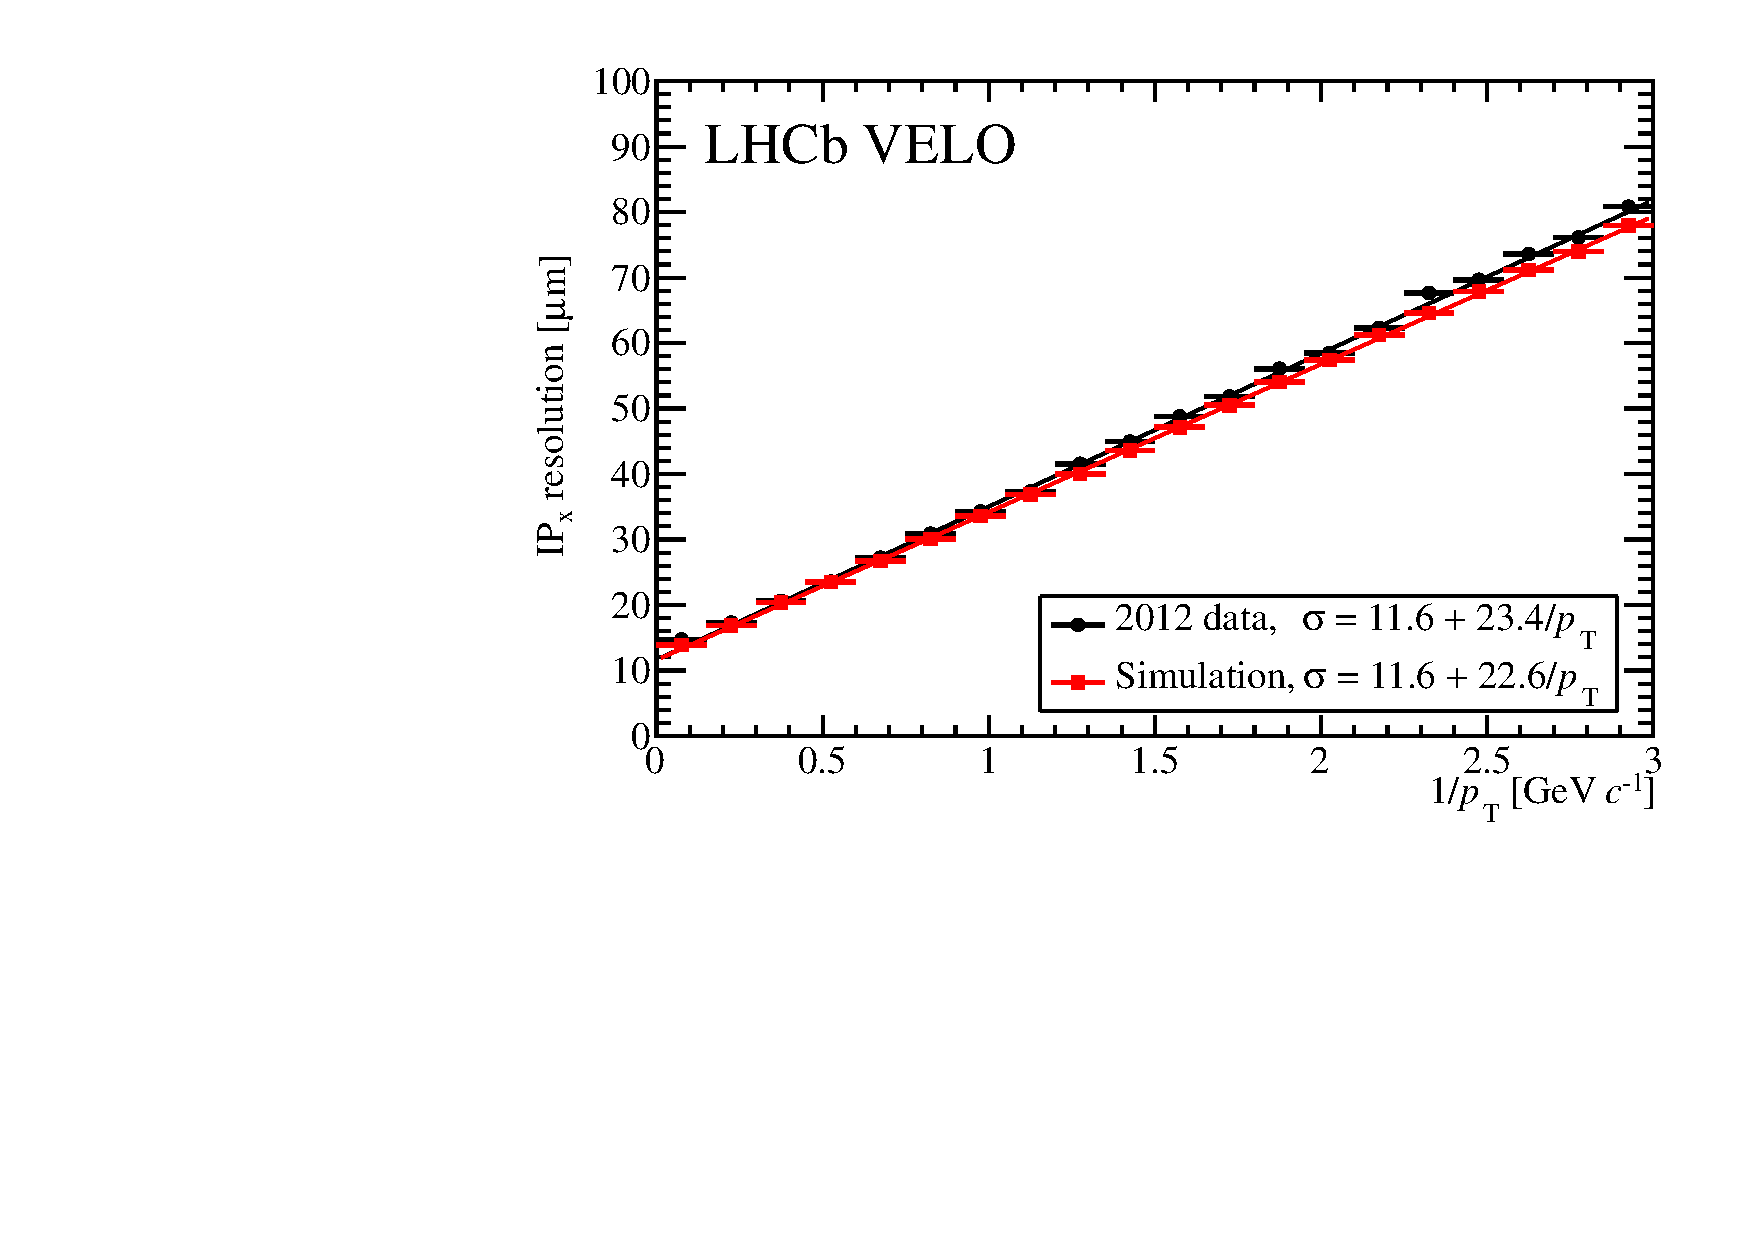
\includegraphics[width=0.48\textwidth]{IPXRes_invp}
    \caption[Impact parameter resolution as a function of inverse transverse momentum comparing
      data and
    simulation]{
      Impact parameter resolution as a function of a track's inverse transverse momentum comparing
      (black)
      data taken in 2012 which is also shown in Fig.~\protect\ref{fig:velo:ipres} and (red)
      simulation.  Excellent agreement is seen, particularly for high momenta tracks,
      $\pt>1\gev$~\protect\cite{LHCb-DP-2014-001}.
    }
    \label{fig:data:ipres}
  \end{center}
\end{figure}




%%%%%%%%%%%%%%%%%%%%%%%%%%%%%%%%%%%%%%%%%%%%%%%%%%%%%%%%%%%%%%%%%%%%%%%%%%%%%%%%

%The high output rate of the \lhcb trigger means that there is a huge amount of data to be made
%accessible to collaborators, too much to be convenient, in fact.
%Because of \lhcb's wide physics program it is possible to run further collaboration wide selection
%twice a year to reduce the dataset by approximately a factor of ten.
%Within each of these data-subsets further stripping flags are applied which further increase the
%speed which a dataset can be processed.
%The stripping lines used in this thesis are the Dimuon line and the







\clearpage
